% =============================================================================
\section{The Objects}\label{sec:objects}
Each object is shown complete and with its parts pulled apart, followed by the basic shapes it uses
and the transformation of every part. For the main objects, the world coordinates of their key parts are
also listed. All tables are produced by the program from the drawing code of the scene.
\Cref{tab:parts} summarises the number of basic shapes of each object.
The world-coordinate tables give, for each key part, two vertices A and B that really exist in the mesh of its
shape (\Cref{tab:vertexpair}); their world position is $\mathbf{p}_{world}=M_{place}\,M_{part}\,\mathbf{v}$.
\begin{table}[H]
\centering\small
\caption{The two mesh vertices A and B listed for each shape (unit-shape coordinates, \Cref{tab:shapes})}\label{tab:vertexpair}
\begin{tabular}{@{}l l l l@{}}
\toprule
Shape & Vertex A & Vertex B & Which vertices \\ \midrule
cube & $(-.5,-.5,-.5)$ & $(.5,.5,.5)$ & opposite corners $v_0$ and $v_6$ (\Cref{fig:cube}) \\
cylinder & $(.5,-.5,0)$ & $(.5,.5,0)$ & first vertex of the bottom ring and of the top ring ($\theta_0=0$) \\
truncated cone & $(.5,-.5,0)$ & $(.35,.5,0)$ & first vertex of the bottom ring and of the top ring \\
cone & $(.5,-.5,0)$ & $(0,.5,0)$ & first vertex of the bottom ring, and the tip \\
sphere & $(0,-.5,0)$ & $(0,.5,0)$ & the two poles ($\phi=\pi$ and $\phi=0$) \\
hemisphere & $(.5,0,0)$ & $(0,.5,0)$ & first vertex of the rim, and the pole \\
torus & $(.5,0,0)$ & $(.3,0,0)$ & outer and inner edge of the tube at $u=0$ \\
wedge & $(-.5,-.5,.5)$ & $(.5,.5,-.5)$ & corners $w_0$ and $w_5$ \\
tapered box & $(-.5,-.5,-.5)$ & $(.35,.5,.3)$ & a bottom corner and a top corner \\
\bottomrule
\end{tabular}
\end{table}


\begin{table}[H]
\centering\scriptsize
\caption{Number of basic shapes per object (Cyl-L / Sph-L = low-poly versions, TCone = truncated cone, TBox = tapered box)}\label{tab:parts}
\setlength{\tabcolsep}{3.0pt}
\begin{tabular}{l r rrrrrrrrrrrrrrr}
\toprule
Object & Total & Cube & Cyl & Cyl-L & Sph & Sph-L & Cone & TCone & Torus & Hemi & Wedge & TBox & Quad & Cross & Leaf & Coil \\
\midrule
Vending machine & \textbf{287} & 79 & 177 & -- & 3 & -- & -- & 16 & -- & -- & -- & -- & -- & -- & -- & 12 \\
ATM & \textbf{49} & 48 & -- & -- & -- & -- & -- & -- & -- & 1 & -- & -- & -- & -- & -- & -- \\
Coffee machine & \textbf{32} & 16 & 9 & -- & 1 & -- & -- & 2 & 4 & -- & -- & -- & -- & -- & -- & -- \\
Television (frame) & \textbf{5} & 4 & -- & -- & 1 & -- & -- & -- & -- & -- & -- & -- & -- & -- & -- & -- \\
Sofa (3 seats) & \textbf{21} & 12 & 9 & -- & -- & -- & -- & -- & -- & -- & -- & -- & -- & -- & -- & -- \\
Armchair & \textbf{13} & 6 & 7 & -- & -- & -- & -- & -- & -- & -- & -- & -- & -- & -- & -- & -- \\
Bookshelf & \textbf{21} & 21 & -- & -- & -- & -- & -- & -- & -- & -- & -- & -- & -- & -- & -- & -- \\
Person (standing) & \textbf{41} & 9 & 11 & -- & 17 & -- & -- & 1 & 1 & 1 & -- & 1 & -- & -- & -- & -- \\
Person (walking) & \textbf{40} & 9 & 11 & -- & 17 & -- & -- & -- & 1 & 1 & -- & 1 & -- & -- & -- & -- \\
Person + chair & \textbf{47} & 15 & 11 & -- & 18 & -- & -- & -- & 1 & 1 & -- & 1 & -- & -- & -- & -- \\
Sedan car + driver & \textbf{115} & 63 & 28 & -- & 18 & -- & -- & -- & 2 & 1 & 1 & 2 & -- & -- & -- & -- \\
SUV + driver & \textbf{117} & 66 & 28 & -- & 18 & -- & -- & -- & 2 & 1 & 1 & 1 & -- & -- & -- & -- \\
Hatchback + driver & \textbf{114} & 62 & 28 & -- & 18 & -- & -- & -- & 2 & 1 & 1 & 2 & -- & -- & -- & -- \\
Rainforest tree & \textbf{27} & -- & -- & 5 & -- & 6 & -- & -- & -- & -- & 4 & -- & -- & -- & 12 & -- \\
Coconut palm & \textbf{37} & -- & -- & 14 & -- & 5 & -- & -- & -- & -- & -- & -- & 18 & -- & -- & -- \\
Bamboo clump & \textbf{130} & -- & -- & 100 & -- & -- & -- & -- & -- & -- & -- & -- & -- & -- & 30 & -- \\
Banana plant & \textbf{28} & -- & -- & 6 & -- & 22 & -- & -- & -- & -- & -- & -- & -- & -- & -- & -- \\
Street lamp & \textbf{5} & 1 & 2 & -- & -- & -- & -- & 1 & -- & -- & -- & 1 & -- & -- & -- & -- \\
Pendant lamp & \textbf{5} & -- & 3 & -- & 1 & -- & -- & 1 & -- & -- & -- & -- & -- & -- & -- & -- \\
Aquarium & \textbf{76} & 12 & -- & 1 & 35 & 6 & 7 & 1 & -- & -- & 7 & -- & -- & 7 & -- & -- \\
6 products & \textbf{23} & 9 & 12 & -- & 1 & -- & -- & 1 & -- & -- & -- & -- & -- & -- & -- & -- \\
Table set & \textbf{23} & 10 & 2 & -- & 3 & 1 & -- & 1 & -- & 1 & -- & -- & -- & -- & 5 & -- \\
Wall clock & \textbf{17} & 14 & 2 & -- & -- & -- & -- & -- & 1 & -- & -- & -- & -- & -- & -- & -- \\
Bush+fern+rock+log & \textbf{23} & -- & -- & 4 & -- & 8 & -- & -- & -- & 3 & -- & -- & 5 & 1 & 2 & -- \\
\bottomrule
\end{tabular}

\end{table}

% =============================================================================
\subsection{Machines}
% -----------------------------------------------------------------------------
\subsubsection{Vending machine}
The vending machine is $1.0\times1.95\times0.8$ m. Its origin is on the floor in the middle and it faces
$+z$. Three machines stand in the lounge: cold drinks (red), crispy snacks (orange) and sweet treats (blue).
\objviews{vending}{Vending machine: (a) complete, (b) disconnected parts with their names.}
\begin{table}[H]\centering\footnotesize
\caption{Vending machine in the world, placed with $M_{place}=T(2.4, 0, -4.5)$: centre of each key part and the world position $M_{place}\,M_{part}\,\mathbf{v}$ of two of its real mesh vertices A and B (\Cref{tab:vertexpair})}\label{tab:world_vending}
\begin{tabular}{@{}l l c c c@{}}
\toprule
Part & Shape & Centre $(x,y,z)$ & Vertex A & Vertex B \\
\midrule
Back panel & cube & $(2.40, 1.00, -4.88)$ & $(1.90, 0.07, -4.90)$ & $(2.90, 1.93, -4.86)$ \\
Side panels (1) & cube & $(1.92, 1.00, -4.50)$ & $(1.90, 0.07, -4.90)$ & $(1.94, 1.93, -4.10)$ \\
Side panels (2) & cube & $(2.88, 1.00, -4.50)$ & $(2.86, 0.07, -4.90)$ & $(2.90, 1.93, -4.10)$ \\
Top panel & cube & $(2.40, 1.93, -4.50)$ & $(1.90, 1.90, -4.90)$ & $(2.90, 1.96, -4.10)$ \\
Base & cube & $(2.40, 0.11, -4.50)$ & $(1.90, 0.04, -4.90)$ & $(2.90, 0.18, -4.10)$ \\
Front glass & cube & $(2.25, 1.22, -4.12)$ & $(1.94, 0.65, -4.12)$ & $(2.56, 1.79, -4.11)$ \\
Keys (1) & cube & $(2.65, 1.50, -4.09)$ & $(2.63, 1.48, -4.10)$ & $(2.68, 1.52, -4.08)$ \\
Keys (2) & cube & $(2.65, 1.44, -4.09)$ & $(2.63, 1.42, -4.10)$ & $(2.68, 1.46, -4.08)$ \\
Collection flap (1) & cube & $(2.25, 0.40, -4.11)$ & $(1.96, 0.23, -4.12)$ & $(2.54, 0.57, -4.10)$ \\
Collection flap (2) & cube & $(2.25, 0.40, -4.10)$ & $(2.14, 0.37, -4.10)$ & $(2.36, 0.43, -4.10)$ \\
Levelling feet (1) & cylinder & $(1.98, 0.03, -4.82)$ & $(2.01, 0.00, -4.82)$ & $(2.01, 0.05, -4.82)$ \\
Levelling feet (2) & cylinder & $(1.98, 0.03, -4.18)$ & $(2.01, 0.00, -4.18)$ & $(2.01, 0.05, -4.18)$ \\
\bottomrule
\end{tabular}
\end{table}


\objhead{Construction.} The machine is a small tree of nodes (\Cref{fig:vendtree}); moving parts are child
nodes whose own transformation changes over time.
\begin{figure}[H]
\centering
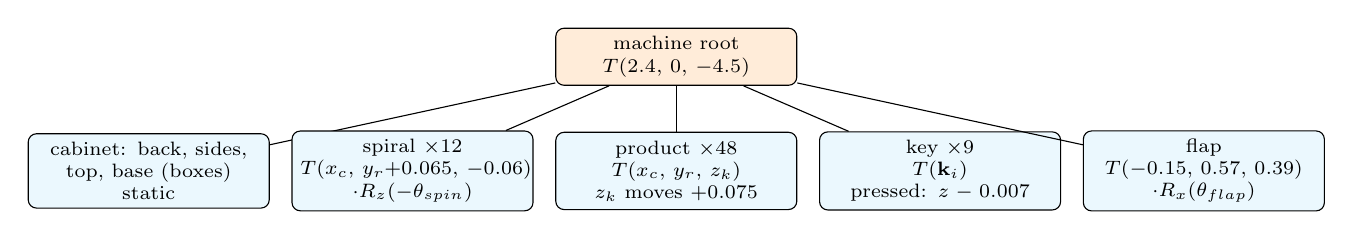
\begin{tikzpicture}[level distance=1.45cm,
  level 1/.style={sibling distance=3.35cm},
  every node/.style={draw,rounded corners=3pt,fill=cyan!8,font=\scriptsize,align=center,inner sep=3pt,text width=2.85cm}]
\node[fill=orange!15] {machine root\\$T(2.4,\,0,\,-4.5)$}
  child {node {cabinet: back, sides,\\top, base (boxes)\\static}}
  child {node {spiral $\times12$\\$T(x_c,\,y_r{+}0.065,\,-0.06)$\\$\cdot R_z(-\theta_{spin})$}}
  child {node {product $\times48$\\$T(x_c,\,y_r,\,z_k)$\\$z_k$ moves $+0.075$}}
  child {node {key $\times9$\\$T(\mathbf{k}_i)$\\pressed: $z-0.007$}}
  child {node {flap\\$T(-0.15,\,0.57,\,0.39)$\\$\cdot R_x(\theta_{flap})$}};
\end{tikzpicture}
\caption{Node tree of the vending machine. Changing $\theta_{spin}$ turns a spiral about its own axis;
changing $\theta_{flap}$ swings the flap about its top edge.}\label{fig:vendtree}
\end{figure}

\emph{Worked example: one vertex of the right side panel, from the unit cube to the world.}
\begin{figure}[H]
\centering
\begin{tikzpicture}[node distance=1.35cm,
  vb/.style={draw,rounded corners=3pt,fill=#1,font=\footnotesize,align=center,minimum height=1.05cm,text width=2.65cm},
  vb/.default=blue!6, lb/.style={font=\scriptsize,above,align=center}]
\node[vb=gray!10] (u) {unit cube\\$v_6=(.5,\,.5,\,.5)$};
\node[vb,right=of u] (s) {scaled\\$(.02,\,.93,\,.40)$};
\node[vb,right=of s] (t) {machine space\\$(.50,\,1.93,\,.40)$};
\node[vb=green!12,right=of t] (w) {world\\$(2.90,\,1.93,\,-4.10)$};
\draw[arr] (u) -- node[lb]{$S(0.04,$\\$1.86,0.8)$} (s);
\draw[arr] (s) -- node[lb]{$T(0.48,$\\$1.0,0)$} (t);
\draw[arr] (t) -- node[lb]{$T(2.4,$\\$0,-4.5)$} (w);
\end{tikzpicture}
\caption{$\mathbf{p}_{world}=T(2.4,0,-4.5)\cdot T(0.48,1.0,0)\cdot S(0.04,1.86,0.8)\cdot\mathbf{v}$ for the corner $v_6$.}\label{fig:vendpipe}
\end{figure}
\begin{table}[H]
\centering\small
\caption{The 8 corners of the vending machine side panel, step by step}\label{tab:vendcorners}
\begin{tabular}{@{}c c c c c@{}}
\toprule
Corner & unit $\mathbf{v}$ & after $S$ & after $T$ (machine space) & world \\ \midrule
$v_0$ & $(-.5,-.5,-.5)$ & $(-.02,-.93,-.40)$ & $(.46,.07,-.40)$ & $(2.86,0.07,-4.90)$ \\
$v_1$ & $(\ .5,-.5,-.5)$ & $(\ .02,-.93,-.40)$ & $(.50,.07,-.40)$ & $(2.90,0.07,-4.90)$ \\
$v_2$ & $(\ .5,\ .5,-.5)$ & $(\ .02,\ .93,-.40)$ & $(.50,1.93,-.40)$ & $(2.90,1.93,-4.90)$ \\
$v_3$ & $(-.5,\ .5,-.5)$ & $(-.02,\ .93,-.40)$ & $(.46,1.93,-.40)$ & $(2.86,1.93,-4.90)$ \\
$v_4$ & $(-.5,-.5,\ .5)$ & $(-.02,-.93,\ .40)$ & $(.46,.07,\ .40)$ & $(2.86,0.07,-4.10)$ \\
$v_5$ & $(\ .5,-.5,\ .5)$ & $(\ .02,-.93,\ .40)$ & $(.50,.07,\ .40)$ & $(2.90,0.07,-4.10)$ \\
$v_6$ & $(\ .5,\ .5,\ .5)$ & $(\ .02,\ .93,\ .40)$ & $(.50,1.93,\ .40)$ & $(2.90,1.93,-4.10)$ \\
$v_7$ & $(-.5,\ .5,\ .5)$ & $(-.02,\ .93,\ .40)$ & $(.46,1.93,\ .40)$ & $(2.86,1.93,-4.10)$ \\
\bottomrule
\end{tabular}
\end{table}
Panel size: $2.86\to2.90$ (4 cm), $0.07\to1.93$ (1.86 m), $-4.90\to-4.10$ (80 cm). The other two machines
use $x=3.7$ and $x=5.0$ in the first translation.

\objhead{Function.} Each machine is a state machine (\Cref{fig:vendsm}). Money is an integer number of Taka.
The user inserts a Tk 10 coin or a Tk 50 note, types a code such as \texttt{B2} (row A--D, column 1--3) and
presses \textbf{OK}. The spiral turns $360^\circ$ in 1.6 s and the products advance by one place (0.075 m).
The front product then falls freely with gravity $g=9.81\,\mathrm{m/s^2}$ and bounces on the tray with a
restitution of 0.32:
\[
v_y \leftarrow v_y - g\,\Delta t,\qquad \mathbf{p}\leftarrow\mathbf{p}+\mathbf{v}\,\Delta t,\qquad
\text{if } p_y < y_{floor}:\ v_y \leftarrow -0.32\,v_y .
\]
When the bounce speed drops below 0.35 m/s the product lies still. Pushing the flap puts it into the
player's bag, the change falls into the coin cup as small coins, and an empty slot is refilled after 40 s.
The LCD, the price tags and the key labels are text drawn on the machine (\Cref{sec:text}).
\begin{figure}[H]
\centering
\begin{tikzpicture}[state/.append style={minimum width=2.5cm,minimum height=1.25cm,font=\footnotesize},lb/.style={font=\scriptsize,align=center}]
\node[state] (idle) at (0,0) {IDLE\\insert money,\\type code};
\node[state] (vend) at (4.7,0) {VENDING\\spiral turns};
\node[state] (drop) at (9.0,0) {DROPPING\\gravity + bounce};
\node[state] (ready) at (13.2,0) {READY\\item in tray};
\draw[arr] (idle) -- node[lb,above]{OK, enough\\credit} (vend);
\draw[arr] (vend) -- node[lb,above]{after 1.6 s} (drop);
\draw[arr] (drop) -- node[lb,above]{at rest} (ready);
\draw[arr] (ready.south) -- ++(0,-0.7) -| node[lb,below,pos=0.25]{push the flap: item goes to the bag, change falls into the cup} (idle.south);
\end{tikzpicture}
\caption{Vending machine state machine.}\label{fig:vendsm}
\end{figure}
\objhead{Colours, textures and sound.} Painted body (red, orange or blue), dark metal trims, steel shelves,
polished metal coin plate and spirals, transparent front glass ($\alpha=0.18$), glowing marquee, tube light
and LEDs. Sounds: a coin sound when money is inserted, the motor while the spiral turns, a thud when the
product hits the tray and small coin sounds when the change lands in the cup.

% -----------------------------------------------------------------------------
\subsubsection{Products}
Every machine holds 12 slots with 4 products each. Six product types exist; their colours come from the
product list of each machine (for example Cola red and white, Mango Juice yellow and green).
\objviews[5.6cm]{products}{Products: can, bottle, juice box, chips bag, chocolate bar and cookie box.}
\objhead{Construction.} A \emph{can} is a cylinder body, a coloured band and two metal rims. A \emph{bottle}
adds a truncated-cone shoulder, a neck and a cap. A \emph{chips bag} is a box with a flattened sphere
(``puff'') and two crimp strips; its round logo is a cylinder rotated $R_x(90^\circ)$. A \emph{chocolate bar}
is a box with a narrower band, a \emph{cookie box} a box with a stripe and a round picture, and a
\emph{juice box} a carton with a label and a straw tilted by $R_z(12^\circ)$.
\objhead{Function.} Products sit on the spirals at $z = 0.0525 - 0.075k$ ($k=0\ldots3$) and move forward while
the spiral turns. A dropped product becomes a free body (position, velocity, spin) until it rests in the tray.
\objhead{Colours, textures and sound.} Two colours per product, glossy plastic for bottles, polished metal
for the can rims. Products have no sounds of their own (the drop sound belongs to the machine).

% -----------------------------------------------------------------------------
\subsubsection{ATM}
The ATM is $1.0\times2.08\times0.72$ m and stands at the back wall of the ATM room.
\objviews{atm}{ATM: (a) complete, (b) disconnected parts with their names.}
\begin{table}[H]\centering\footnotesize
\caption{ATM in the world, placed with $M_{place}=T(-9.5, 0, -4.55)$: centre of each key part and the world position $M_{place}\,M_{part}\,\mathbf{v}$ of two of its real mesh vertices A and B (\Cref{tab:vertexpair})}\label{tab:world_atm}
\begin{tabular}{@{}l l c c c@{}}
\toprule
Part & Shape & Centre $(x,y,z)$ & Vertex A & Vertex B \\
\midrule
Plinth & cube & $(-9.50, 0.04, -4.55)$ & $(-10.00, 0.00, -4.91)$ & $(-9.00, 0.08, -4.19)$ \\
Lower cabinet & cube & $(-9.50, 0.54, -4.55)$ & $(-9.98, 0.08, -4.88)$ & $(-9.02, 1.00, -4.22)$ \\
Upper fascia & cube & $(-9.50, 1.45, -4.63)$ & $(-9.98, 1.05, -4.88)$ & $(-9.02, 1.85, -4.38)$ \\
Header & cube & $(-9.50, 1.96, -4.55)$ & $(-10.02, 1.84, -4.91)$ & $(-8.98, 2.08, -4.19)$ \\
Screen & cube & $(-9.50, 1.46, -4.36)$ & $(-9.71, 1.30, -4.36)$ & $(-9.29, 1.62, -4.36)$ \\
Keypad shelf (tilted) (1) & cube & $(-9.50, 1.03, -4.15)$ & $(-9.98, 1.04, -4.30)$ & $(-9.02, 1.03, -4.00)$ \\
Keypad shelf (tilted) (2) & cube & $(-9.50, 1.06, -4.15)$ & $(-9.68, 1.09, -4.27)$ & $(-9.32, 1.04, -4.04)$ \\
Cash dispenser (1) & cube & $(-9.50, 0.88, -4.21)$ & $(-9.70, 0.83, -4.22)$ & $(-9.30, 0.93, -4.21)$ \\
Cash dispenser (2) & cube & $(-9.50, 0.88, -4.20)$ & $(-9.66, 0.86, -4.21)$ & $(-9.34, 0.90, -4.20)$ \\
Card slot (1) & cube & $(-9.16, 1.30, -4.37)$ & $(-9.22, 1.27, -4.38)$ & $(-9.10, 1.33, -4.36)$ \\
Card slot (2) & cube & $(-9.16, 1.30, -4.35)$ & $(-9.21, 1.30, -4.36)$ & $(-9.11, 1.30, -4.35)$ \\
\bottomrule
\end{tabular}
\end{table}

\objhead{Construction.} A plinth, a lower cabinet and an upper fascia (boxes) carry the screen bezel, the
card slot, the receipt slot, the cash dispenser and two privacy wings. The keypad shelf is a child node
tilted towards the user,
\[
M_{keypad} = M_{ATM}\cdot T(0,\,1.035,\,0.40)\cdot R_x(12^\circ),
\]
and the 16 keys are placed in that node on a $4\times4$ grid,
$\mathbf{k}_i = (-0.135 + 0.075\,(i \bmod 4),\ 0.03,\ -0.085 + 0.052\,\lfloor i/4\rfloor)$, so they follow the slope
automatically. A pressed key moves down by 6 mm. The card slides in and out along $z$, four bank notes slide
out of the dispenser, and the receipt is a thin box rotated by $R_x(25^\circ\cdot a)$ while it comes out.
\objhead{Function.} The ATM follows the state machine of \Cref{fig:atmsm}. The PIN is 1234; amounts of
Tk 500, 1,000, 2,000, 5,000 (side keys), fast cash or any other multiple of 100 can be withdrawn. The card is
always returned before the cash, and the cash is added to the player's wallet and taken from the bank
balance. The screen shows every step with rectangles and text, and a panel on the HUD lists the eight steps
(\Cref{sec:interaction}).
\objhead{Colours, textures and sound.} Dark grey cabinet, light grey fascia, blue header with a glowing light
strip, brushed metal keypad plate, coloured CANCEL / CLEAR / ENTER keys, glowing screen. Sounds: a beep for
every key and a cash-counting sound when the notes come out.

% -----------------------------------------------------------------------------
\subsubsection{Coffee machine}
The coffee machine ($0.43\times0.81\times0.40$ m) stands on the counter in the lounge.
\objviews{coffee}{Coffee machine while brewing: (a) complete, (b) disconnected parts with their names.}
\begin{table}[H]\centering\footnotesize
\caption{Coffee machine in the world, placed with $M_{place}=T(-5, 0.92, -4.55)$: centre of each key part and the world position $M_{place}\,M_{part}\,\mathbf{v}$ of two of its real mesh vertices A and B (\Cref{tab:vertexpair})}\label{tab:world_coffee}
\begin{tabular}{@{}l l c c c@{}}
\toprule
Part & Shape & Centre $(x,y,z)$ & Vertex A & Vertex B \\
\midrule
Base & cube & $(-5.00, 0.94, -4.55)$ & $(-5.20, 0.92, -4.75)$ & $(-4.80, 0.96, -4.35)$ \\
Steel column & cube & $(-5.00, 1.24, -4.65)$ & $(-5.20, 0.96, -4.75)$ & $(-4.80, 1.52, -4.55)$ \\
Head unit & cube & $(-5.00, 1.45, -4.55)$ & $(-5.21, 1.37, -4.75)$ & $(-4.79, 1.53, -4.35)$ \\
Bean hopper & truncated cone & $(-5.00, 1.62, -4.61)$ & $(-4.88, 1.71, -4.61)$ & $(-4.92, 1.53, -4.61)$ \\
Drip tray + grill (1) & cube & $(-5.00, 0.97, -4.47)$ & $(-5.14, 0.96, -4.56)$ & $(-4.86, 0.98, -4.38)$ \\
Drip tray + grill (2) & cube & $(-5.11, 0.98, -4.47)$ & $(-5.11, 0.98, -4.55)$ & $(-5.11, 0.98, -4.39)$ \\
Cup & truncated cone & $(-5.00, 1.03, -4.46)$ & $(-4.96, 1.07, -4.46)$ & $(-4.97, 0.98, -4.46)$ \\
\bottomrule
\end{tabular}
\end{table}

\objhead{Construction.} A base, a steel column, two side panels and a head unit form the body. The bean
hopper is a glass truncated cone turned upside down with $R_x(180^\circ)$, so it is wider at the top. The three
round buttons are cylinders rotated $R_x(90^\circ)$ so that their flat face points forward, each with a torus ring.
The cup is also an upside-down truncated cone with a torus handle. The coffee inside the cup is a thin disc whose
height and radius follow the cup's taper:
\[
h = 0.006 + 0.075\,f,\qquad r = 2\,\big(0.0298 + (0.0425-0.0298)\,h/0.09\big) - 0.006,
\]
where $f\in[0,1]$ is the fill level. The pouring stream is a thin cylinder from the nozzle down to the
coffee surface.
\objhead{Function.} The three buttons make an Espresso, a Cappuccino or a Masala Tea:
\texttt{IDLE} $\rightarrow$ \texttt{CUP\_DROP} (0.5 s, the cup falls) $\rightarrow$ \texttt{GRINDING} (1.6 s) $\rightarrow$
\texttt{BREWING} (4.5 s, the cup fills) $\rightarrow$ \texttt{READY}. Steam puffs rise from the cup (\Cref{sec:particles}).
Taking the cup puts the drink into the bag.
\objhead{Colours, textures and sound.} Black body, brushed steel column, glass hopper with brown bean texture,
glowing LCD and status LED (green when idle, orange while busy). Sounds: grinder, pouring and a beep when ready.

% -----------------------------------------------------------------------------
\subsubsection{Television}
The television hangs on the lounge wall at $(0,1.75,-4.86)$.
\objviews[6.5cm]{tv}{Television: (a) complete with the news channel, (b) disconnected parts.}
\begin{table}[H]\centering\footnotesize
\caption{Television in the world, placed with $M_{place}=T(0, 1.75, -4.86)$: centre of each key part and the world position $M_{place}\,M_{part}\,\mathbf{v}$ of two of its real mesh vertices A and B (\Cref{tab:vertexpair})}\label{tab:world_tv}
\begin{tabular}{@{}l l c c c@{}}
\toprule
Part & Shape & Centre $(x,y,z)$ & Vertex A & Vertex B \\
\midrule
Wall bracket & cube & $(0.00, 1.75, -4.92)$ & $(-0.23, 1.59, -4.95)$ & $(0.23, 1.91, -4.89)$ \\
TV body & cube & $(0.00, 1.75, -4.88)$ & $(-0.93, 1.21, -4.90)$ & $(0.93, 2.29, -4.85)$ \\
Screen & cube & $(0.00, 1.75, -4.85)$ & $(-0.89, 1.25, -4.85)$ & $(0.89, 2.25, -4.85)$ \\
Bottom trim & cube & $(0.00, 1.20, -4.86)$ & $(-0.93, 1.19, -4.88)$ & $(0.93, 1.21, -4.83)$ \\
Power LED & sphere & $(0.86, 1.22, -4.84)$ & $(0.86, 1.21, -4.84)$ & $(0.86, 1.22, -4.84)$ \\
\bottomrule
\end{tabular}
\end{table}

\objhead{Construction.} A wall bracket, a body box, a bottom trim, the screen and a power LED. The pictures
are not textures: each channel is drawn every frame on a \emph{canvas} placed on the screen, using
rectangles and text. Circles (heads, the sun, trees, the ball) are drawn as horizontal strips of width
$2\sqrt{r^2-y^2}$, and triangles (mountains) as strips whose width shrinks linearly with the height.
\objhead{Function.} Looking at the screen and pressing E cycles through news (with a moving ticker), nature,
live football and a weather map that shows the in-game time, and off. While it is on, the TV adds a
flickering coloured point light to the room whose colour follows the picture.
\objhead{Colours, textures and sound.} Black body, dark metal bracket, glowing screen, green or red power
LED. A click is heard when the channel changes.

% -----------------------------------------------------------------------------
\subsubsection{Aquarium and fish}
The aquarium ($1.8\times1.45\times0.5$ m) stands in the library.
\objviews{aquarium}{Aquarium: (a) complete, (b) disconnected parts (stand, sand, rocks, plants, glass, water, fish, bubbles).}
\begin{table}[H]\centering\footnotesize
\caption{Aquarium in the world, placed with $M_{place}=T(9.8, 0, 4.45)\,R_y(180^\circ)$: centre of each key part and the world position $M_{place}\,M_{part}\,\mathbf{v}$ of two of its real mesh vertices A and B (\Cref{tab:vertexpair})}\label{tab:world_aquarium}
\begin{tabular}{@{}l l c c c@{}}
\toprule
Part & Shape & Centre $(x,y,z)$ & Vertex A & Vertex B \\
\midrule
Wooden stand & cube & $(9.80, 0.38, 4.45)$ & $(10.70, 0.00, 4.70)$ & $(8.90, 0.75, 4.20)$ \\
Sand bed & cube & $(9.80, 0.79, 4.45)$ & $(10.68, 0.76, 4.68)$ & $(8.92, 0.82, 4.22)$ \\
Water & cube & $(9.80, 1.03, 4.45)$ & $(10.68, 0.78, 4.68)$ & $(8.92, 1.28, 4.22)$ \\
Glass tank & cube & $(9.80, 1.06, 4.45)$ & $(10.70, 0.75, 4.70)$ & $(8.90, 1.37, 4.20)$ \\
Hood & cube & $(9.80, 1.41, 4.45)$ & $(10.72, 1.37, 4.72)$ & $(8.88, 1.45, 4.18)$ \\
Fish bodies (1) & sphere & $(10.19, 1.06, 4.45)$ & $(10.19, 1.04, 4.45)$ & $(10.19, 1.09, 4.45)$ \\
Fish bodies (2) & sphere & $(9.39, 1.12, 4.46)$ & $(9.39, 1.10, 4.46)$ & $(9.39, 1.15, 4.46)$ \\
\bottomrule
\end{tabular}
\end{table}

\objhead{Construction.} A wooden stand with three doors carries a sand bed, rocks (squashed low spheres), a
driftwood branch (low cylinder rotated $R_y(30^\circ)R_z(75^\circ)$), water plants (cross cards), an air stone,
the water volume and the glass tank (two transparent boxes) and a hood with a light strip. Each fish is a node
$T(x,y,z)\cdot R_y(\psi)$ with a sphere body scaled to $(0.45s,0.75s,1.25s)$, a cone tail in a child node that
wags with $R_y(25^\circ\sin(9t+3\varphi))$, a wedge fin and two sphere eyes.
\objhead{Function.} Each of the 7 fish swims on its own ellipse, $x=r_x\cos\varphi$, $z=r_z\sin\varphi$ with
$\varphi \mathrel{+}= \omega\,\Delta t$, and faces its direction of motion, $\psi=\operatorname{atan2}(\Delta x,\Delta z)$.
``Feed the fish'' drops 12 food crumbs that sink slowly; while there is food, every fish swims up to the
surface. Bubbles rise from the air stone and the plants sway (\Cref{sec:effects}).
\objhead{Colours, textures and sound.} Wood texture on the stand, sand texture, rock texture, bark texture on
the driftwood, transparent water ($\alpha=0.16$) and glass, glowing hood light. A click sounds when the fish
are fed.

% =============================================================================
\subsection{Furniture}
% -----------------------------------------------------------------------------
\subsubsection{Sofa}
The sofa function builds a sofa for any number of seats $n$; its width is $W = 0.72n + 0.32$ m. The lounge
has two three-seat sofas and four armchairs.
\objviews{sofa}{Sofa with three seats: (a) complete, (b) disconnected parts.}
\begin{table}[H]\centering\footnotesize
\caption{Sofa (3 seats) in the world, placed with $M_{place}=T(0, 0, -0.6)\,R_y(180^\circ)$: centre of each key part and the world position $M_{place}\,M_{part}\,\mathbf{v}$ of two of its real mesh vertices A and B (\Cref{tab:vertexpair})}\label{tab:world_sofa}
\begin{tabular}{@{}l l c c c@{}}
\toprule
Part & Shape & Centre $(x,y,z)$ & Vertex A & Vertex B \\
\midrule
Base frame & cube & $(0.00, 0.20, -0.60)$ & $(1.24, 0.09, -0.16)$ & $(-1.24, 0.31, -1.04)$ \\
Back frame & cube & $(0.00, 0.56, -0.23)$ & $(1.24, 0.23, -0.15)$ & $(-1.24, 0.89, -0.31)$ \\
Seat cushions (1) & cube & $(0.72, 0.38, -0.65)$ & $(1.07, 0.30, -0.33)$ & $(0.37, 0.46, -0.97)$ \\
Seat cushions (2) & cube & $(0.00, 0.38, -0.65)$ & $(0.35, 0.30, -0.33)$ & $(-0.35, 0.46, -0.97)$ \\
Arm rests (1) & cube & $(1.16, 0.42, -0.60)$ & $(1.24, 0.20, -0.16)$ & $(1.08, 0.64, -1.04)$ \\
Arm rests (2) & cube & $(-1.16, 0.42, -0.60)$ & $(-1.08, 0.20, -0.16)$ & $(-1.24, 0.64, -1.04)$ \\
Legs (1) & cylinder & $(1.16, 0.04, -0.24)$ & $(1.14, 0.00, -0.24)$ & $(1.14, 0.09, -0.24)$ \\
Legs (2) & cylinder & $(1.16, 0.04, -0.96)$ & $(1.14, 0.00, -0.96)$ & $(1.14, 0.09, -0.96)$ \\
\bottomrule
\end{tabular}
\end{table}

\objhead{Construction.} A base frame and a back frame (boxes); per seat a cushion box, a rounded front roll
(cylinder rotated $R_z(90^\circ)$ so that it lies along $x$) and a back cushion tilted by $R_x(-10^\circ)$; two
arm rests made of a box and a rolled cylinder rotated $R_x(90^\circ)$ to lie along $z$; four wooden legs; and
two throw pillows rotated about all three axes.
\objhead{Function.} Visitors can sit on any seat: each seat has a stand point and a sit point. The sitting
pose of a person is described in \Cref{sec:humans}.
\objhead{Colours, textures and sound.} Blue fabric texture (darker on the frame), yellow fabric pillows, wooden
legs. No sound.

% -----------------------------------------------------------------------------
\subsubsection{Armchair}
\objviews[6.5cm]{armchair}{Armchair: (a) complete, (b) disconnected parts.}
\objhead{Construction and function.} The armchair is the sofa function called with $n=1$ (no throw pillows),
which shows how one parametric model produces different objects. Armchairs stand in the lounge and in the
library, where visitors sit and read.
\objhead{Colours, textures and sound.} Brown fabric texture, wooden legs. No sound.

% -----------------------------------------------------------------------------
\subsubsection{Coffee table and rug}
\objviews[6.5cm]{tableset}{Coffee table on its rug: (a) complete, (b) disconnected parts.}
\objhead{Construction.} A wooden top and a lower shelf (boxes), four metal legs placed at
$(\pm(w/2-0.06),\,0.2,\,\pm(d/2-0.06))$, two magazines rotated about $y$, a fruit bowl and three fruits. The bowl
is a hemisphere scaled with a \emph{negative} $y$ factor, $S=(0.24,-0.10,0.24)$, which mirrors it so that it opens
upwards. The rug is two thin boxes: a border and a carpet-textured centre.
\objhead{Colours, textures and sound.} Wood texture, dark metal legs, carpet texture on the rug. No sound.

% -----------------------------------------------------------------------------
\subsubsection{Bookshelf}
\objviews{bookshelf}{Bookshelf: (a) complete, (b) disconnected parts.}
\begin{table}[H]\centering\footnotesize
\caption{Bookshelf in the world, placed with $M_{place}=T(9, 0, -4.69)$: centre of each key part and the world position $M_{place}\,M_{part}\,\mathbf{v}$ of two of its real mesh vertices A and B (\Cref{tab:vertexpair})}\label{tab:world_bookshelf}
\begin{tabular}{@{}l l c c c@{}}
\toprule
Part & Shape & Centre $(x,y,z)$ & Vertex A & Vertex B \\
\midrule
Side boards (1) & cube & $(8.12, 1.15, -4.69)$ & $(8.10, 0.00, -4.88)$ & $(8.14, 2.30, -4.50)$ \\
Side boards (2) & cube & $(9.88, 1.15, -4.69)$ & $(9.86, 0.00, -4.88)$ & $(9.90, 2.30, -4.50)$ \\
Top board & cube & $(9.00, 2.28, -4.69)$ & $(8.10, 2.26, -4.88)$ & $(9.90, 2.30, -4.50)$ \\
Back board & cube & $(9.00, 1.15, -4.87)$ & $(8.10, 0.00, -4.88)$ & $(9.90, 2.30, -4.86)$ \\
Shelves (1) & cube & $(9.00, 0.10, -4.69)$ & $(8.13, 0.09, -4.87)$ & $(9.87, 0.11, -4.51)$ \\
Shelves (2) & cube & $(9.00, 0.54, -4.69)$ & $(8.13, 0.52, -4.87)$ & $(9.87, 0.55, -4.51)$ \\
Plinth & cube & $(9.00, 0.05, -4.69)$ & $(8.10, 0.00, -4.88)$ & $(9.90, 0.10, -4.50)$ \\
\bottomrule
\end{tabular}
\end{table}

\objhead{Construction.} Two side boards, a top, a back board, a plinth and five shelves. The books are not
modelled one by one: each row is a plain box (the colour of the pages) with a quad in front that carries the
generated \emph{books} texture. Each shelf has two rows of different widths, and on every second shelf one
quad is mirrored with a negative $x$ scale, so the pattern does not repeat. One book leans by $R_z(-12^\circ)$.
\objhead{Function.} Visitors stand in front of the shelves and browse.
\objhead{Colours, textures and sound.} Wood texture, books texture, plain page colour. No sound.

% -----------------------------------------------------------------------------
\subsubsection{Reading table and chair}
\objviews[6.5cm]{reading}{Reading table and chair: (a) complete, (b) disconnected parts.}
\objhead{Construction.} The table is a round top, a pedestal and a foot disc (cylinders) with a book box
rotated by $R_y(20^\circ)$. The chair is a seat box, a backrest tilted by $R_x(-6^\circ)$ and four legs at
$(\pm0.19,\,0.21,\,\pm0.19)$; in the figure the chair node is turned by $R_y(180^\circ)$ to face the table.
\objhead{Colours, textures and sound.} Wood texture, dark metal pedestal, red fabric seat. No sound.

% -----------------------------------------------------------------------------
\subsubsection{Wall clock}
Three clocks hang in the building; their hands show the in-game time.
\objviews[6.0cm]{clock}{Wall clock: (a) complete, (b) disconnected parts.}
\begin{table}[H]\centering\footnotesize
\caption{Wall clock in the world, placed with $M_{place}=T(0, 3, -4.87)$: centre of each key part and the world position $M_{place}\,M_{part}\,\mathbf{v}$ of two of its real mesh vertices A and B (\Cref{tab:vertexpair})}\label{tab:world_clock}
\begin{tabular}{@{}l l c c c@{}}
\toprule
Part & Shape & Centre $(x,y,z)$ & Vertex A & Vertex B \\
\midrule
Wooden rim & torus & $(0.00, 3.00, -4.85)$ & $(0.21, 3.00, -4.85)$ & $(0.13, 3.00, -4.85)$ \\
Clock face & cylinder & $(0.00, 3.00, -4.86)$ & $(0.18, 3.00, -4.87)$ & $(0.18, 3.00, -4.84)$ \\
Hour hand & cube & $(-0.04, 3.03, -4.83)$ & $(0.00, 2.99, -4.84)$ & $(-0.08, 3.06, -4.83)$ \\
Minute hand & cube & $(0.04, 3.06, -4.83)$ & $(-0.01, 3.00, -4.83)$ & $(0.09, 3.11, -4.83)$ \\
Centre cap & cylinder & $(0.00, 3.00, -4.83)$ & $(0.01, 3.00, -4.83)$ & $(0.01, 3.00, -4.82)$ \\
\bottomrule
\end{tabular}
\end{table}

\objhead{Construction.} A torus rim and a face disc, both rotated $R_x(90^\circ)$ to face forward. Each of the
12 ticks is a box in its own node rotated by $R_z(-30^\circ\,i)$, so the same box is repeated around the face.
The hands are boxes in nodes rotated by
\[
\theta_{hour} = -30^\circ\cdot(h \bmod 12),\qquad \theta_{minute} = -6^\circ\cdot m,
\]
where $h$ is the in-game hour (with fraction) and $m$ the minutes.
\objhead{Colours, textures and sound.} Wooden rim, light face, dark ticks and hands, red centre cap. No sound.

% -----------------------------------------------------------------------------
\subsubsection{Pendant lamp}
\objviews[6.5cm]{pendant}{Pendant lamp: (a) complete, (b) disconnected parts.}
\objhead{Construction.} A ceiling disc, a cord (thin cylinder), a shade (truncated cone), a diffuser disc and a
bulb sphere. The lamp node is placed at the ceiling point and every part hangs below it, so the cord length is
one parameter.
\objhead{Function.} Each lamp belongs to a light group. When the group is on, the bulb and the diffuser glow
and a point light is placed at the bulb (\Cref{sec:lighting}).
\objhead{Colours, textures and sound.} Dark (lounge) or bronze (library) shade, glowing bulb. No sound.

% -----------------------------------------------------------------------------
\subsubsection{Table lamp and floor lamp}
\objviews[6.5cm]{lamps}{Table lamp on a side table, and a floor lamp: (a) complete, (b) disconnected parts.}
\objhead{Construction.} The table lamp is a ceramic base (sphere), a stem and a fabric shade (truncated cone);
the side table is a round top, a stem and a foot disc. The floor lamp is a base disc, a 1.6 m pole, a shade
and a bulb.
\objhead{Function.} The table lamps belong to the lounge light group; the floor lamp is the reading lamp of the
library and belongs to the spot-light group. When on, the shades glow warm white.
\objhead{Colours, textures and sound.} Fabric shades, dark metal, polished metal stem. No sound.

% -----------------------------------------------------------------------------
\subsubsection{Potted plants}
\objviews[6.5cm]{plants}{The three potted plants: (a) complete, (b) disconnected parts.}
\objhead{Construction.} Every pot is a truncated cone turned upside down ($R_x(180^\circ)$) with a soil disc.
Variant 0 has a stem, a dark core sphere and five leaf cards turned by $R_y(72^\circ\,i)$; variant 1 has six fern
fronds (quads tilted $R_x(35^\circ)$ and turned $R_y(60^\circ\,i)$) and a cross card; variant 2 (snake plant)
has seven thin cones turned by $R_y(51^\circ\,i)$ and tilted $\pm6^\circ$.
\objhead{Colours, textures and sound.} White or terracotta pots, leaf, fern and plain green materials. No sound.

% -----------------------------------------------------------------------------
\subsubsection{Counter and wall cabinet}
\objviews[6.5cm]{counter}{Kitchen counter with a wall cabinet: (a) complete, (b) disconnected parts.}
\objhead{Construction.} The counter is a cabinet body, a black toe kick, a marble top and $\max(2,\lfloor w/0.6\rfloor)$
doors with handles; the handles alternate between the left and right edge of the doors. The wall cabinet
uses the same rule. The coffee machine stands on this counter.
\objhead{Colours, textures and sound.} Wood texture, marble texture, polished metal handles. No sound.

% -----------------------------------------------------------------------------
\subsubsection{Bench}
\objviews[6.0cm]{bench}{Outdoor bench: (a) complete, (b) disconnected parts.}
\objhead{Construction.} Two metal side frames, two back supports tilted by $R_x(-10^\circ)$, four seat slats and
two back slats with the same tilt. Two benches stand on the sidewalk.
\objhead{Colours, textures and sound.} Wood texture slats, dark metal frame. No sound.

% -----------------------------------------------------------------------------
\subsubsection{Waste bin}
\objviews[6.0cm]{bin}{Waste bin: (a) complete, (b) disconnected parts.}
\objhead{Construction.} A cylinder body, a hemisphere lid, a box for the opening and a foot ring. Bins stand
outside next to the benches and inside the building.
\objhead{Colours, textures and sound.} Polished stainless steel, which shows a bright specular highlight
(\Cref{sec:lighting}). No sound.

% -----------------------------------------------------------------------------
\subsubsection{Light switch}
\objviews[5.5cm]{switch}{Light switch: (a) complete, (b) disconnected parts.}
\objhead{Construction.} A plate, a rocker tilted by $R_x(\mp15^\circ)$ depending on the state, and an indicator
LED sphere.
\objhead{Function.} Six switches on the walls control the light groups (lounge, spot lights, ATM room,
library, outdoor). Looking at a switch highlights it; pressing E toggles its group and the rocker flips
(\Cref{sec:interaction}).
\objhead{Colours, textures and sound.} White plastic, green LED when on and red when off. A click is heard.

% -----------------------------------------------------------------------------
\subsubsection{Security camera}
\objviews[5.5cm]{camera}{Security camera: (a) complete, (b) disconnected parts.}
\objhead{Construction.} A wall mount, an arm tilted by $R_x(20^\circ)$ and a camera node
$T(0,-0.10,0.24)\cdot R_x(25^\circ)\,R_y(30^\circ\sin 0.4t)$ that holds the body, the lens and a recording LED.
\objhead{Function.} The camera slowly pans left and right; its LED blinks once per second.
\objhead{Colours, textures and sound.} White plastic, black lens, red glowing LED. No sound.

% -----------------------------------------------------------------------------
\subsubsection{Paintings}
\objviews[5.0cm]{painting}{The three wall paintings: (a) complete, (b) disconnected parts.}
\objhead{Construction.} A wooden frame box and a picture made of flat shapes: a landscape (sky, hills as a
hemisphere rotated $R_x(90^\circ)$, a sun disc), abstract blocks, and a jungle sunset with five flattened cones
as trees.
\objhead{Colours, textures and sound.} Matte colours, wood frame. No sound.

% -----------------------------------------------------------------------------
\subsubsection{Sliding entrance doors}
\objviews[6.5cm]{doors}{Automatic sliding doors (closed): (a) complete, (b) disconnected parts.}
\begin{table}[H]\centering\footnotesize
\caption{Sliding doors in the world, placed with $M_{place}=T(0, 0, 5.18)$: centre of each key part and the world position $M_{place}\,M_{part}\,\mathbf{v}$ of two of its real mesh vertices A and B (\Cref{tab:vertexpair})}\label{tab:world_doors}
\begin{tabular}{@{}l l c c c@{}}
\toprule
Part & Shape & Centre $(x,y,z)$ & Vertex A & Vertex B \\
\midrule
Glass pane (1) & cube & $(-0.60, 1.30, 5.18)$ & $(-1.20, 0.08, 5.17)$ & $(0.00, 2.52, 5.19)$ \\
Glass pane (2) & cube & $(0.60, 1.30, 5.18)$ & $(0.00, 0.08, 5.17)$ & $(1.20, 2.52, 5.19)$ \\
Top and bottom rails (1) & cube & $(-0.60, 2.55, 5.18)$ & $(-1.22, 2.50, 5.16)$ & $(0.02, 2.60, 5.21)$ \\
Top and bottom rails (2) & cube & $(-0.60, 0.05, 5.18)$ & $(-1.22, 0.00, 5.16)$ & $(0.02, 0.10, 5.21)$ \\
Edge posts (1) & cube & $(0.00, 1.30, 5.18)$ & $(-0.02, 0.10, 5.16)$ & $(0.02, 2.50, 5.21)$ \\
Edge posts (2) & cube & $(0.00, 1.30, 5.18)$ & $(-0.02, 0.10, 5.16)$ & $(0.02, 2.50, 5.21)$ \\
Handles (1) & cube & $(-0.10, 1.05, 5.22)$ & $(-0.12, 0.80, 5.21)$ & $(-0.09, 1.30, 5.24)$ \\
Handles (2) & cube & $(0.10, 1.05, 5.22)$ & $(0.09, 0.80, 5.21)$ & $(0.12, 1.30, 5.24)$ \\
\bottomrule
\end{tabular}
\end{table}

\objhead{Construction.} Each leaf is a glass pane, a top and a bottom rail, an edge post and a handle. The left
leaf is drawn in the node $T(-x_{off},0,z)$ and the right leaf in $T(+x_{off},0,z)$, with
\[
x_{off} = 0.6 + 1.15\cdot o,
\]
where $o\in[0,1]$ is the opening.
\objhead{Function.} The doors open while a person (the player or a visitor) is within $2.2\times2.8$ m of the
entrance, $o$ moving towards its target at 1.6 per second. While they are closed they block the way.
\objhead{Colours, textures and sound.} Transparent glass, dark metal rails, polished metal handles. A short
whoosh is heard when the doors start to move.

% -----------------------------------------------------------------------------
\subsubsection{Ceiling and roof fixtures}
\objviews[5.5cm]{fixtures}{Roof air conditioner, recessed spot light, tube light and smoke detector (the ceiling fixtures are turned to face the viewer): (a) complete, (b) disconnected parts.}
\objhead{Construction.} The air conditioner is a casing box, a fan opening (disc), a torus fan guard and a
grille. The spot light is a torus ring around a glowing lens; the tube light is a housing box with two glowing
tubes (cylinders rotated $R_z(90^\circ)$); the smoke detector is a disc with a small LED.
\objhead{Function.} Spot and tube lights glow when their light group is on and carry the spot and point lights
of the rooms.
\objhead{Colours, textures and sound.} Light grey plastic, polished metal rings, glowing lenses. No sound.

% -----------------------------------------------------------------------------
\subsubsection{Street lamp and bollard}
\objviews{streetlamp}{Street lamp and a sidewalk bollard: (a) complete, (b) disconnected parts.}
\begin{table}[H]\centering\footnotesize
\caption{Street lamp + bollard in the world, placed with $M_{place}=T(-18, 0, 8.25)$: centre of each key part and the world position $M_{place}\,M_{part}\,\mathbf{v}$ of two of its real mesh vertices A and B (\Cref{tab:vertexpair})}\label{tab:world_streetlamp}
\begin{tabular}{@{}l l c c c@{}}
\toprule
Part & Shape & Centre $(x,y,z)$ & Vertex A & Vertex B \\
\midrule
Concrete base & cylinder & $(-18.00, 0.15, 8.25)$ & $(-17.83, 0.00, 8.25)$ & $(-17.83, 0.30, 8.25)$ \\
Tapered pole & truncated cone & $(-18.00, 2.90, 8.25)$ & $(-17.91, 0.00, 8.25)$ & $(-17.94, 5.80, 8.25)$ \\
Arm & cylinder & $(-18.00, 5.75, 8.80)$ & $(-17.97, 5.75, 8.25)$ & $(-17.97, 5.75, 9.35)$ \\
Lamp head & tapered box & $(-18.00, 5.74, 9.40)$ & $(-18.19, 5.81, 9.71)$ & $(-17.87, 5.67, 9.21)$ \\
Glowing lens & cube & $(-18.00, 5.66, 9.40)$ & $(-18.15, 5.65, 9.15)$ & $(-17.85, 5.67, 9.65)$ \\
\bottomrule
\end{tabular}
\end{table}

\objhead{Construction.} The street lamp is a concrete base, a tapered pole (truncated cone) of height
$h=5.8$ m, an arm (cylinder rotated $R_x(90^\circ)$), a lamp head (tapered box rotated $R_x(180^\circ)$ so that it
is wider at the top) and a glowing lens. The bollard is a post, a light ring and a hemisphere cap.
\objhead{Function.} The outdoor lamps switch on automatically at dusk. Each street lamp carries a point light that stays
on at any distance.
\objhead{Colours, textures and sound.} Concrete texture, dark metal, warm sodium-coloured glow. No sound.

% -----------------------------------------------------------------------------
\subsubsection{The building}
\begin{figure}[H]
\centering
\begin{minipage}{0.52\linewidth}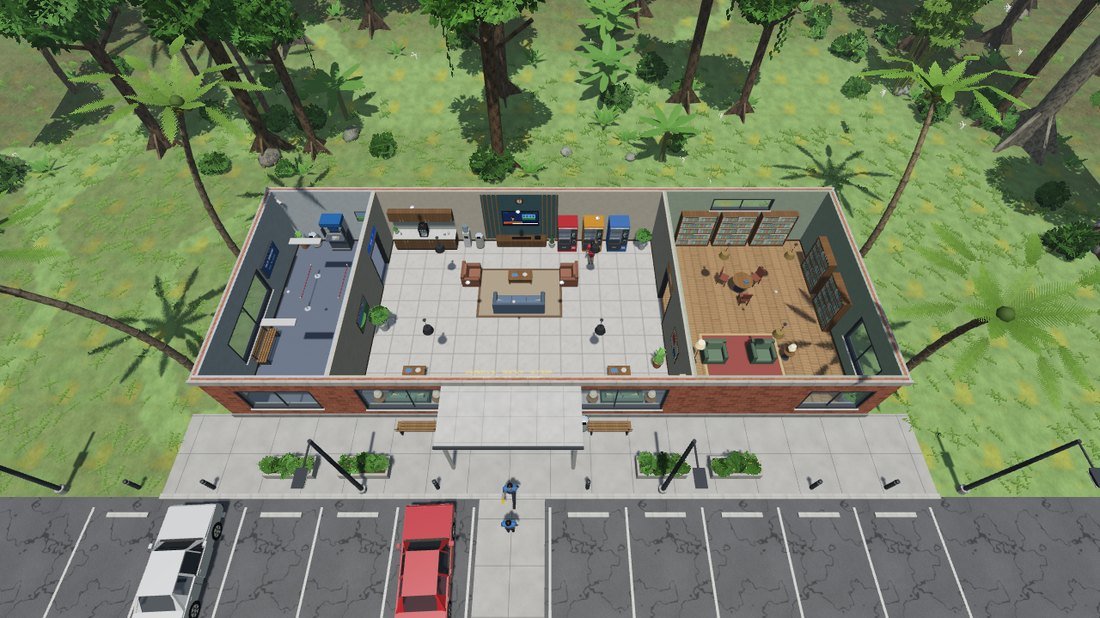
\includegraphics[width=\linewidth]{cutaway_day}\end{minipage}\hfill
\begin{minipage}{0.45\linewidth}
\centering
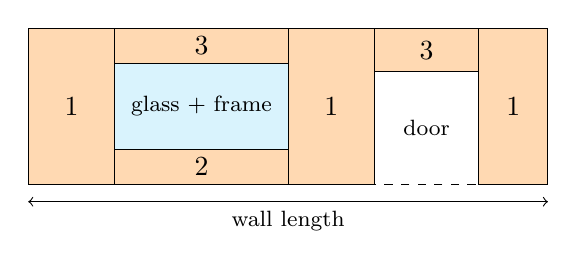
\begin{tikzpicture}[x=0.55cm,y=0.55cm]
\draw[fill=orange!30] (0,0) rectangle (2,3.6); \node at (1,1.8) {1};
\draw[fill=orange!30] (2,0) rectangle (6,0.8); \node at (4,0.4) {2};
\draw[fill=cyan!15] (2,0.8) rectangle (6,2.8); \node[font=\footnotesize] at (4,1.8) {glass + frame};
\draw[fill=orange!30] (2,2.8) rectangle (6,3.6); \node at (4,3.2) {3};
\draw[fill=orange!30] (6,0) rectangle (8,3.6); \node at (7,1.8) {1};
\draw[fill=orange!30] (8,2.6) rectangle (10.4,3.6); \node at (9.2,3.1) {3};
\draw[dashed] (8,0) rectangle (10.4,2.6); \node[font=\footnotesize] at (9.2,1.3) {door};
\draw[fill=orange!30] (10.4,0) rectangle (12,3.6); \node at (11.2,1.8) {1};
\draw[<->] (0,-0.4) -- (12,-0.4) node[midway,below,font=\footnotesize]{wall length};
\end{tikzpicture}
\end{minipage}
\caption{Left: the building with the roof hidden. Right: a wall with one window and one door is split into
(1) full pieces, (2) a piece below the window and (3) pieces above the openings.}\label{fig:wall}
\end{figure}
\objhead{Construction.} All walls are made by one function, \texttt{buildWall()}, which takes a straight wall
and a list of openings and splits the wall into boxes: full-height pieces between openings, a piece below each
window, a lintel above each opening, and for a window a glass pane, an aluminium frame (four bars and a
mullion) and a marble sill; for a door, frame trims. Every piece has two half-thickness layers: brick outside
and plaster inside, in the colour of the room (beige lounge, light blue ATM room, sage green library). Wooden
skirting boards run along the floor. The floors are tiles (lounge), carpet (ATM room) and wood (library).
The roof, the parapet, two air conditioners and the sign board are drawn per frame, so that the roof can be
hidden in the cut-away view.
\objhead{Colours, textures and sound.} Brick, plaster, floor tile, carpet, wood, ceiling tile, roof and
concrete textures.

% =============================================================================
\subsection{People}\label{sec:humans}
There are two types of person, a man and a woman, built by the same function with the same hierarchy
(\Cref{fig:humangraph}); only a few sizes, the hair style and the colours differ. The player's own body is the man.
\begin{figure}[H]
\centering
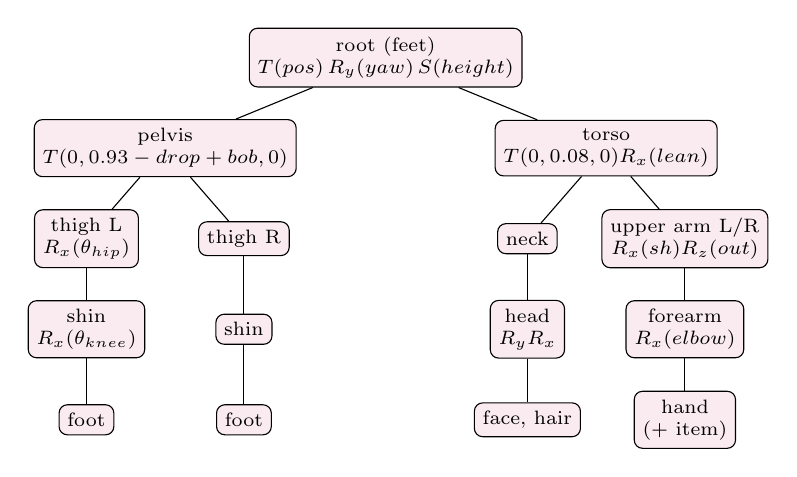
\begin{tikzpicture}[level distance=1.15cm,
  level 1/.style={sibling distance=5.6cm},level 2/.style={sibling distance=2.0cm},level 3/.style={sibling distance=1.9cm},
  every node/.style={draw,rounded corners=3pt,fill=purple!8,font=\scriptsize,align=center,inner sep=3pt}]
\node {root (feet)\\$T(pos)\,R_y(yaw)\,S(height)$}
  child {node {pelvis\\$T(0,0.93-drop+bob,0)$}
     child {node {thigh L\\$R_x(\theta_{hip})$} child {node {shin\\$R_x(\theta_{knee})$} child {node {foot}}}}
     child {node {thigh R} child {node {shin} child {node{foot}}}}}
  child {node {torso\\$T(0,0.08,0)R_x(lean)$}
     child {node {neck} child {node {head\\$R_y R_x$} child {node{face, hair}}}}
     child {node {upper arm L/R\\$R_x(sh)R_z(out)$} child {node {forearm\\$R_x(elbow)$} child {node{hand\\(+ item)}}}}};
\end{tikzpicture}
\caption{Scene graph of a person. A pose only changes the joint angles; every body part stays attached to its parent.}\label{fig:humangraph}
\end{figure}

% -----------------------------------------------------------------------------
\subsubsection{Man}
\objviews{human_walk}{The man (standing): (a) complete, (b) disconnected parts with their names.}
\begin{table}[H]\centering\footnotesize
\caption{Man in the world, placed with $M_{place}=T(0, 0, 6)\,R_y(180^\circ)$: centre of each key part and the world position $M_{place}\,M_{part}\,\mathbf{v}$ of two of its real mesh vertices A and B (\Cref{tab:vertexpair})}\label{tab:world_human_walk}
\begin{tabular}{@{}l l c c c@{}}
\toprule
Part & Shape & Centre $(x,y,z)$ & Vertex A & Vertex B \\
\midrule
Pelvis & cylinder & $(0.00, 0.95, 6.00)$ & $(-0.17, 0.86, 6.00)$ & $(-0.17, 1.04, 6.00)$ \\
Chest & tapered box & $(0.00, 1.31, 6.00)$ & $(-0.21, 1.46, 6.12)$ & $(0.15, 1.16, 5.93)$ \\
Head & sphere & $(0.00, 1.64, 6.00)$ & $(0.00, 1.52, 6.00)$ & $(0.00, 1.76, 6.00)$ \\
Thighs (1) & truncated cone & $(0.09, 0.68, 6.00)$ & $(0.01, 0.90, 6.00)$ & $(0.03, 0.45, 6.00)$ \\
Thighs (2) & truncated cone & $(-0.09, 0.68, 6.00)$ & $(-0.18, 0.90, 6.00)$ & $(-0.15, 0.45, 6.00)$ \\
Shins (1) & truncated cone & $(0.09, 0.24, 6.00)$ & $(0.02, 0.45, 6.00)$ & $(0.04, 0.03, 6.00)$ \\
Shins (2) & truncated cone & $(-0.09, 0.24, 6.00)$ & $(-0.16, 0.45, 6.00)$ & $(-0.14, 0.03, 6.00)$ \\
Upper arms (1) & truncated cone & $(0.24, 1.29, 6.00)$ & $(0.17, 1.42, 6.00)$ & $(0.22, 1.14, 6.00)$ \\
Upper arms (2) & truncated cone & $(-0.24, 1.29, 6.00)$ & $(-0.28, 1.44, 6.00)$ & $(-0.29, 1.15, 6.00)$ \\
Shoes (1) & cube & $(0.09, 0.01, 5.96)$ & $(0.15, -0.03, 6.08)$ & $(0.04, 0.04, 5.83)$ \\
Shoes (2) & cylinder & $(0.09, 0.01, 5.83)$ & $(0.04, 0.04, 5.83)$ & $(0.15, 0.04, 5.83)$ \\
\bottomrule
\end{tabular}
\end{table}

\objhead{Construction.} Every joint is a sphere and every limb a truncated cone. The cones are flipped with
$R_x(180^\circ)$, so the legs are thicker at the hip and the arms thicker at the shoulder. The chest is a tapered
box rotated by $R_z(180^\circ)$ (wide at the shoulders), the waist an elliptic cylinder. The face has sphere eyes,
pupils, nose, ears and jaw and box eyebrows and mouth; the short hair is a hemisphere and a sphere.

\emph{Worked example: the knee.} The knee of the left leg is found by following the chain of nodes:
\[
\mathbf{p}_{knee} = \underbrace{T(\mathbf{p})R_y(\psi)}_{\text{person}}\cdot
\underbrace{T(0,0.93,0)}_{\text{pelvis}}\cdot
\underbrace{T(0.092,-0.03,0)\,R_x(\theta_{thigh})}_{\text{hip}}\cdot
\underbrace{T(0,-0.45,0)}_{\text{knee}}\cdot(0,0,0,1)^T,
\]
with $R_x(\theta):(x,y,z)\mapsto(x,\ y\cos\theta - z\sin\theta,\ y\sin\theta + z\cos\theta)$. In person space:
\begin{itemize}
  \item standing, $\theta_{thigh}=0$: knee at $(0.092,\ 0.90-0.45,\ 0) = (0.092,\ 0.45,\ 0)$;
  \item walking, leg forward, $\theta_{thigh}=-26^\circ$: $(0.092,\ 0.90-0.45\cos26^\circ,\ 0.45\sin26^\circ) = (0.092,\ 0.496,\ 0.197)$.
\end{itemize}
The knee moves 20 cm forward and 4.6 cm up, and the shin and the foot follow because they are its children.

\objhead{Function (animation).} Only the joint angles change. For walking with the phase $\varphi$
($\varphi \mathrel{+}= 7\,\Delta t$):
\[
\theta_{thigh}^{L,R} = \mp 26^\circ\sin\varphi,\quad
\theta_{knee}^{L} = 38^\circ\max(0,\cos\varphi)+4^\circ,\quad
\theta_{shoulder}^{L,R} = \pm22^\circ\sin\varphi,\quad
bob = 0.035\,(1-|\sin\varphi|).
\]
Sitting lowers the pelvis by 0.44 m, turns the thighs by $-88^\circ$ and bends the knees by $88^\circ$. Driving,
pressing buttons and bending down are further fixed poses. Every angle is blended linearly over 0.35 s, so
changes between poses are smooth.
\objhead{Colours, textures and sound.} Skin colour, blue fabric shirt, dark fabric trousers, dark shoes with
white soles, black hair. Footsteps are silent.

% -----------------------------------------------------------------------------
\subsubsection{Woman}
\objviews{human}{The woman holding a coffee cup: (a) complete, (b) disconnected parts with their names.}
\objhead{Construction.} The same hierarchy with a root scale $S(0.95)$ and a width factor $w=0.94$ (her hip is at
$x=0.092\cdot0.94=0.086$). The long hair adds a tall flattened sphere behind the head. She wears a kurta: the
pelvis uses the shirt colour and a hem (an upside-down truncated cone) covers the upper legs. A held item (cup,
can, snack or phone) is a child of the right hand.
\begin{figure}[H]
\centering
\begin{subfigure}{0.3\linewidth}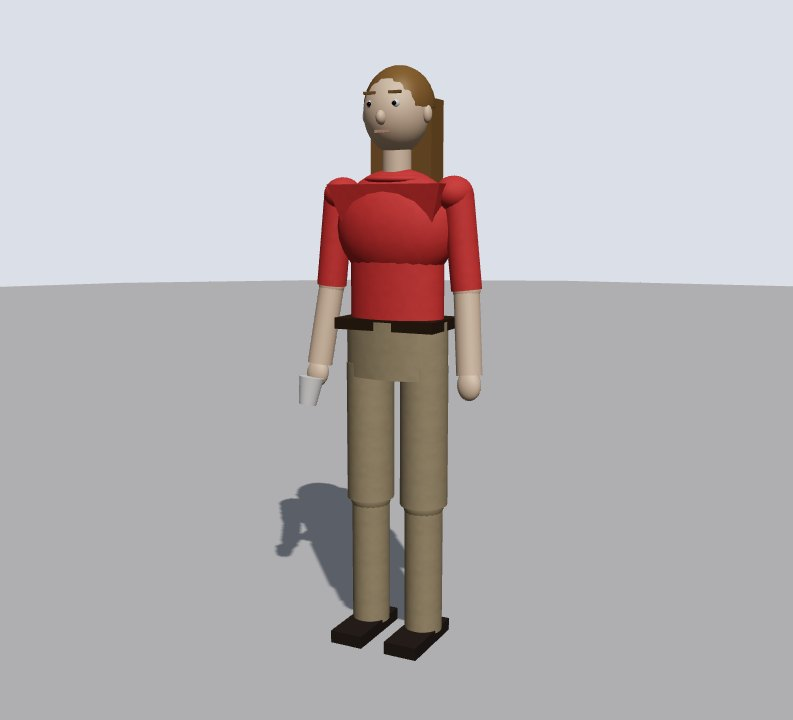
\includegraphics[width=\linewidth]{obj_human}\caption{Standing with a cup}\end{subfigure}
\begin{subfigure}{0.3\linewidth}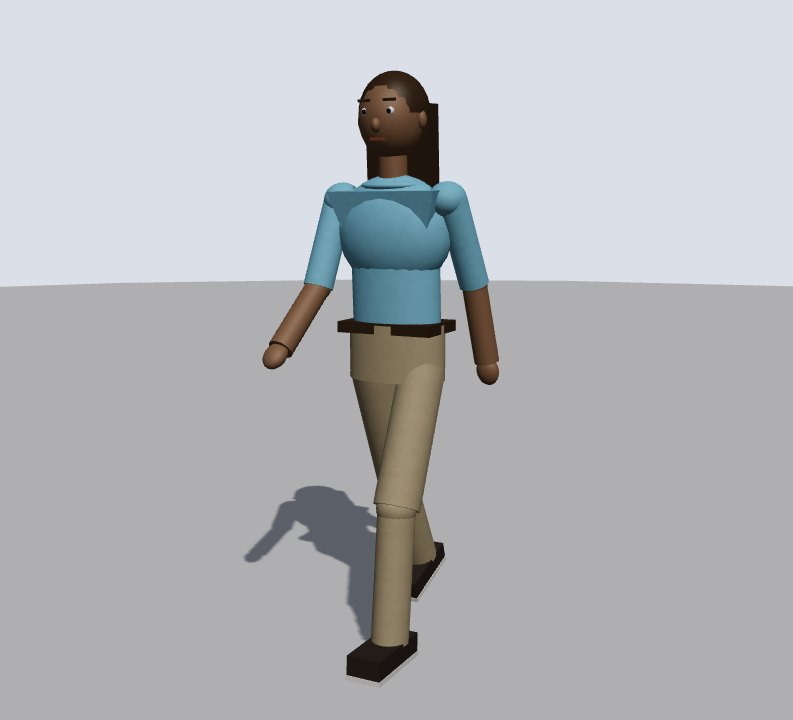
\includegraphics[width=\linewidth]{obj_human_walk}\caption{Walking pose}\end{subfigure}
\begin{subfigure}{0.3\linewidth}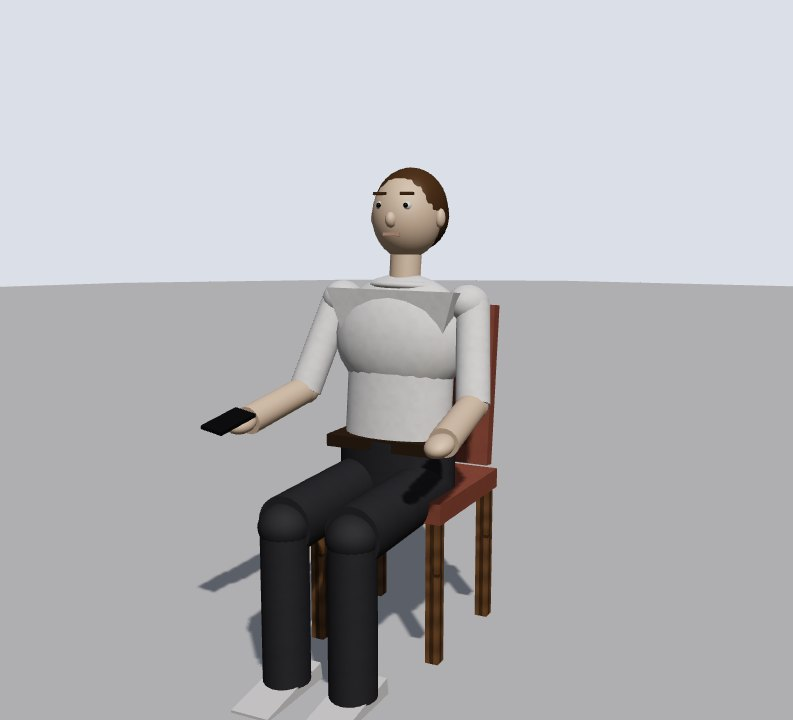
\includegraphics[width=\linewidth]{obj_human_sit}\caption{Sitting on a chair}\end{subfigure}
\caption{Poses produced by the same hierarchical model.}
\end{figure}
\objhead{Colours, textures and sound.} Red kurta, light trousers, brown shoes, long black hair.

% =============================================================================
\subsection{Car}
There is one car model, a sedan of $4.4\times1.78\times1.42$ m, painted red, blue or white.
\objviews[6.5cm]{car_red}{The car (driver door open $55^\circ$, front wheels steered $18^\circ$): (a) complete with its driver, (b) disconnected parts.}
\begin{table}[H]\centering\footnotesize
\caption{Car in the world, placed with $M_{place}=T(-3, 0, 11.2)$: centre of each key part and the world position $M_{place}\,M_{part}\,\mathbf{v}$ of two of its real mesh vertices A and B (\Cref{tab:vertexpair})}\label{tab:world_car_red}
\begin{tabular}{@{}l l c c c@{}}
\toprule
Part & Shape & Centre $(x,y,z)$ & Vertex A & Vertex B \\
\midrule
Front block & cube & $(-3.00, 0.58, 12.64)$ & $(-3.89, 0.30, 11.93)$ & $(-2.11, 0.86, 13.35)$ \\
Rear block & cube & $(-3.00, 0.58, 9.99)$ & $(-3.89, 0.30, 9.05)$ & $(-2.11, 0.86, 10.93)$ \\
Roof & cube & $(-3.00, 1.39, 11.00)$ & $(-3.59, 1.36, 10.29)$ & $(-2.41, 1.42, 11.71)$ \\
Bonnet (wedge) & wedge & $(-3.00, 0.90, 12.78)$ & $(-3.86, 0.86, 13.35)$ & $(-2.14, 0.94, 12.20)$ \\
Windscreen & cube & $(-3.00, 1.12, 11.92)$ & $(-3.57, 0.86, 12.15)$ & $(-2.43, 1.38, 11.69)$ \\
Tyres (1) & cylinder & $(-3.78, 0.32, 12.53)$ & $(-3.68, 0.64, 12.49)$ & $(-3.88, 0.64, 12.56)$ \\
Tyres (2) & cylinder & $(-2.22, 0.32, 12.53)$ & $(-2.12, 0.64, 12.49)$ & $(-2.32, 0.64, 12.56)$ \\
Driver door (1) & cube & $(-4.32, 0.58, 11.65)$ & $(-4.74, 0.32, 11.38)$ & $(-3.90, 0.85, 11.92)$ \\
Driver door (2) & cube & $(-4.30, 0.58, 11.62)$ & $(-4.70, 0.33, 11.36)$ & $(-3.90, 0.83, 11.88)$ \\
\bottomrule
\end{tabular}
\end{table}

\objhead{Construction.} The body is a front block and a rear block (boxes), a passenger-side skin and a floor,
with a rounded nose (cylinder rotated $R_z(90^\circ)$), bumpers and an underbody. The bonnet is a wedge sloping to
the front. The windscreen, the rear window and the side windows are thin parallelograms and triangles built
directly from their corner points (\Cref{sec:transform}); pillars are beams between two points. Inside are
seats, a rear bench, a dashboard and a steering wheel (torus rotated $R_x(70^\circ)$).

\emph{Worked example: a tyre.} The tyre is a cylinder with $S=(0.64,0.22,0.64)$ rotated by $R_z(90^\circ)$, so its
axis points sideways, inside the wheel node $T(-0.78,0.32,1.325)$. With $R_z(90^\circ):(x,y,z)\mapsto(-y,x,z)$:
\begin{table}[H]
\centering\small
\caption{Three vertices of the front tyre (car space)}
\begin{tabular}{@{}l c c c c@{}}
\toprule
Vertex & unit $\mathbf{p}$ & after $S$ & after $R_z(90^\circ)$ & after wheel $T$ \\ \midrule
$\mathbf{p}_0^{top}$ & $(0.5,0.5,0)$ & $(0.32,0.11,0)$ & $(-0.11,0.32,0)$ & $(-0.89,0.64,1.325)$ \\
$\mathbf{p}_0^{bot}$ & $(0.5,-0.5,0)$ & $(0.32,-0.11,0)$ & $(0.11,0.32,0)$ & $(-0.67,0.64,1.325)$ \\
$\mathbf{p}_6^{top}$ & $(0,0.5,0.5)$ & $(0,0.11,0.32)$ & $(-0.11,0,0.32)$ & $(-0.89,0.32,1.645)$ \\
\bottomrule
\end{tabular}
\end{table}
The top of the tyre is at $y=0.64$, twice the wheel radius, so the tyre touches the ground at $y=0$. When the
car moves, the spin $R_x(\theta_{spin})$, the steering $R_y(\delta)$ (front wheels) and the car's own
$T(\mathbf{p}_{car})R_y(\psi)$ are added.

\emph{Worked example: the driver door.} The door is a child node $T(\mathbf{h})\cdot R_y(\theta_{door})$ with the
hinge $\mathbf{h}=(-0.905,0,0.73)$. Its outer panel has $S=(0.04,0.534,1.0)$ and $T=(-0.01,0.582,-0.5)$, so the
rear-bottom corner $v_0$ is at $(-0.03,0.315,-1.0)$ in door space. With
$R_y(\theta): x'=x\cos\theta+z\sin\theta,\ z'=-x\sin\theta+z\cos\theta$:
\begin{itemize}
  \item door closed, $\theta=0^\circ$: $(-0.03,0.315,-1.0)+\mathbf{h} = (-0.935,\ 0.315,\ -0.27)$;
  \item door open, $\theta=70^\circ$: $(-0.950,\ 0.315,\ -0.314)+\mathbf{h} = (-1.855,\ 0.315,\ 0.416)$.
\end{itemize}
The back edge swings 92 cm out while the points on the hinge line stay fixed. The door glass is a child of
the door node, so it swings with the door.

\objhead{Function.} The wheels turn with $\theta_{spin} \mathrel{+}= \Delta s/R$, where $\Delta s$ is the distance driven,
and the front wheels steer with $\delta = \arctan\!\big(L_{wb}\,\Delta\psi/\Delta s\big)$ ($L_{wb}$ = wheel base,
$\Delta\psi$ = change of heading). Headlights, tail and brake lights, reverse lights and blinking indicators
follow the driving state; at night the headlights are real spot lights. How the cars drive is explained in
\Cref{sec:npc}.
\begin{figure}[H]
\centering
\begin{subfigure}{0.32\linewidth}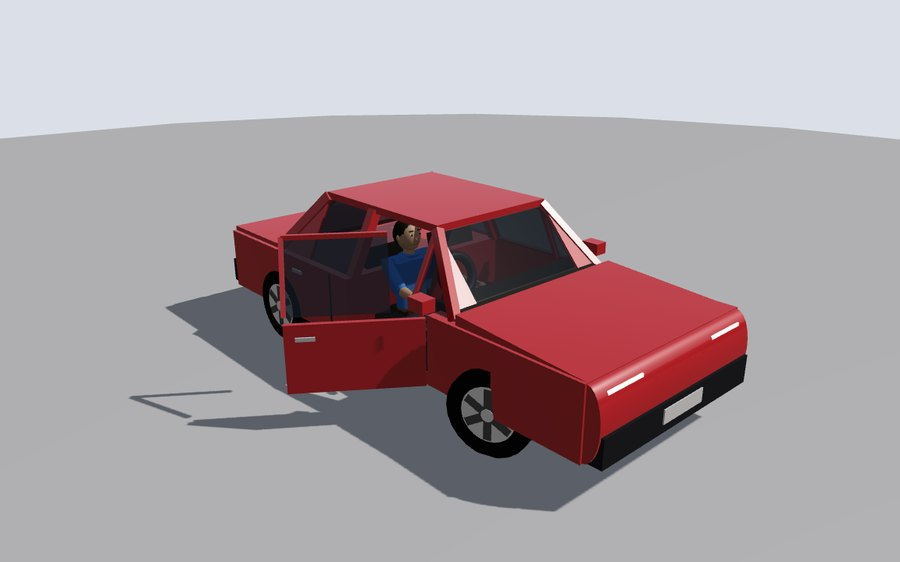
\includegraphics[width=\linewidth]{obj_car_red}\caption{Red}\end{subfigure}
\begin{subfigure}{0.32\linewidth}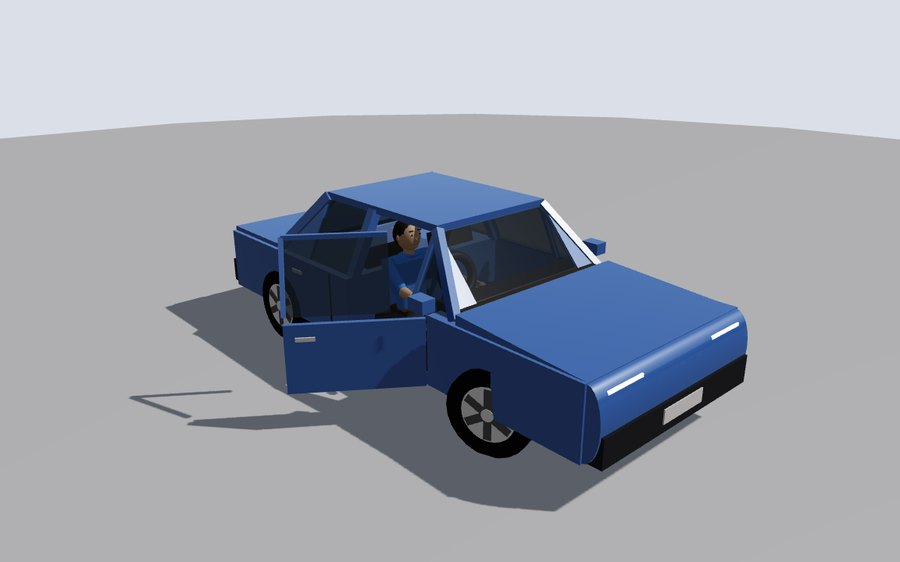
\includegraphics[width=\linewidth]{obj_car_blue}\caption{Blue}\end{subfigure}
\begin{subfigure}{0.32\linewidth}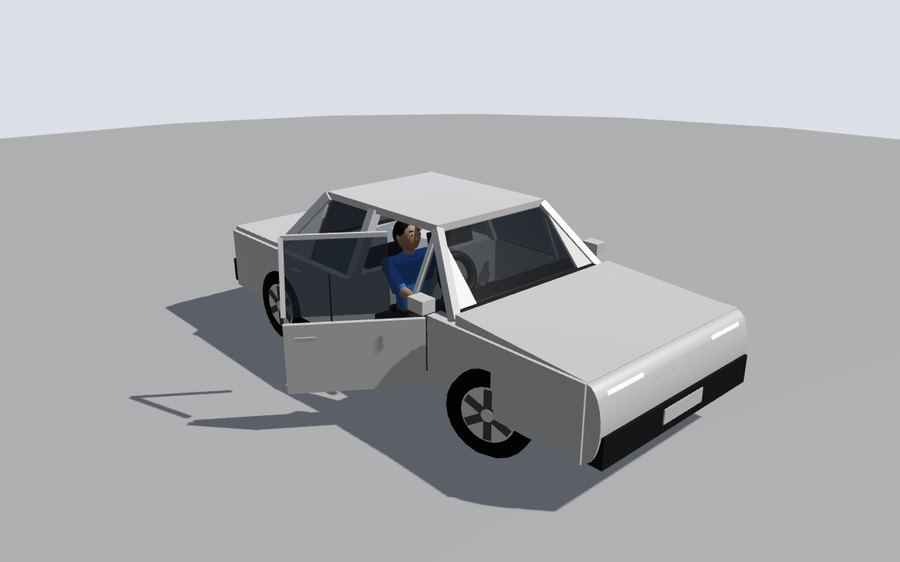
\includegraphics[width=\linewidth]{obj_car_white}\caption{White}\end{subfigure}
\caption{The car model in its three paint colours.}
\end{figure}
\objhead{Colours, textures and sound.} Glossy car paint, tinted transparent glass ($\alpha=0.45$), black rubber
tyres, polished metal rims and handles, glowing lights. Sounds: the door opening and closing when a visitor
gets in or out.

% =============================================================================
\subsection{Jungle}
% -----------------------------------------------------------------------------
\subsubsection{Rainforest tree}
\objviews{tree}{Rainforest tree: (a) complete, (b) disconnected parts.}
\objhead{Construction.} A low-poly trunk (6.5--9 m) and an upper trunk, four buttress roots (wedges), three
branches in nodes $R_y(yaw)\,R_x(45^\circ\ldots60^\circ)$, sometimes a hanging vine, and a crown: three dark core
blobs inside give the crown volume, and 15--19 alpha-tested leaf cards, each turned randomly about all three
axes, are placed on an ellipsoid shell around the crown centre $\mathbf{c}$:
\[
\mathbf{p} = \mathbf{c} + k\,(\cos\alpha\sqrt{1-y^2}\,r_x,\ y\,r_y,\ \sin\alpha\sqrt{1-y^2}\,r_z),\qquad
\alpha\in[0,2\pi),\ y\in[-0.55,1],\ k\in[0.55,1].
\]

\emph{Worked example: a buttress root.} Fin $i$ is a wedge with $S=(0.13,1.5,1.2)$ and $T=(0,0.75,0.6)$ inside a
node turned by $R_y(90^\circ i)$. For $i=1$: the bottom-front vertex $w_0=(-.5,-.5,.5)$ becomes $(-0.065,-0.75,0.6)$
after $S$, $(-0.065,0,1.2)$ after $T$, and $(1.2,\ 0,\ 0.065)$ after $R_y(90^\circ)$; the top-back vertex
$w_2=(-.5,.5,-.5)$ becomes $(0,\ 1.5,\ 0.065)$. Each fin therefore starts on the trunk 1.5 m above the ground and
reaches the ground 1.2 m away from it.
\objhead{Colours, textures and sound.} Bark texture, leaf-cluster cut-out texture, every card with a slightly
different green. Birds sing in the background by day (\Cref{sec:sound}).

% -----------------------------------------------------------------------------
\subsubsection{Coconut palm}
\objviews{palm}{Coconut palm: (a) complete, (b) disconnected parts.}
\objhead{Construction.} The trunk is a chain of seven segments. Each segment is a child of the previous one with
an extra $R_x(3^\circ\ldots7^\circ)$, so the rotations add up and the trunk bends smoothly:
$M_{k+1} = M_k\cdot T(0,L,0)\cdot R_x(\beta)$. Each segment has a ring. The crown has a heart (sphere), nine fronds made
of two quads (the outer half is a child of the inner half and droops by another $30^\circ\ldots45^\circ$) and four coconuts.
\objhead{Colours, textures and sound.} Bark texture, palm frond cut-out texture.

% -----------------------------------------------------------------------------
\subsubsection{Emergent tree}
\objviews{emergent}{Emergent giant tree: (a) complete, (b) disconnected parts.}
\objhead{Construction.} A 14--18 m trunk, five large buttress roots turned by $R_y(72^\circ\,i)$, four branches and
a wide, flat crown made of 20--24 leaf cards on a flattened ellipsoid ($r_x=r_z=4.2$, $r_y=1.3$). These trees
rise above the rest of the forest.
\objhead{Colours, textures and sound.} Light bark texture, leaf-cluster texture.

% -----------------------------------------------------------------------------
\subsubsection{Bamboo clump}
\objviews{bamboo}{Bamboo clump: (a) complete, (b) disconnected parts.}
\objhead{Construction.} 9--15 culms (thin low-poly cylinders) in nodes with a random position on a disc and a
small random tilt $R(\pm8^\circ,\ \text{random yaw},\ \pm8^\circ)$, node rings every 1.3 m and two leaf cards per culm.
\objhead{Colours, textures and sound.} Plain green culms, leaf-cluster texture.

% -----------------------------------------------------------------------------
\subsubsection{Banana plant}
\objviews{banana}{Banana plant: (a) complete, (b) disconnected parts.}
\objhead{Construction.} One to three pseudo-stems (cylinders); at the top of each, 5--8 long leaves are spheres
squashed to $(0.55,0.04,1.9)$ and turned by $R_y(360^\circ\,l/n)\,R_x(-35^\circ\ldots15^\circ)$. Some plants carry a
bunch of bananas on a stalk.
\objhead{Colours, textures and sound.} Matte greens; the leaves use two-sided foliage lighting.

% -----------------------------------------------------------------------------
\subsubsection{Undergrowth}
\objviews{undergrowth}{Undergrowth: a bush, a fern, a rock and a fallen log: (a) complete, (b) disconnected parts.}
\objhead{Construction.} A bush is a dark core sphere and 5--7 leaf cards (sometimes with flowers). A fern is
five quads tilted by $R_x(55^\circ)$ and turned by $R_y(72^\circ\,i)$ plus a cross card. A rock is 1--3 squashed
low spheres with random rotations. A fallen log is a horizontal cylinder ($R_z(90^\circ)$) with moss blobs and
mushrooms made of a cylinder stem and a hemisphere cap.
\objhead{Colours, textures and sound.} Leaf, fern, rock and bark textures.

% -----------------------------------------------------------------------------
\subsubsection{Bird}
\objviews[5.5cm]{bird}{Bird: (a) complete, (b) disconnected parts.}
\objhead{Construction.} A body (squashed sphere), a cone beak rotated $R_x(90^\circ)$ and two wings. Each wing is a
box in a child node rotated by $R_z(\pm\phi)$ about the body axis, with $\phi = 35^\circ\sin(\text{flap})$, so the two
wings flap symmetrically.
\objhead{Function.} Nine birds fly on circles above the jungle by day (\Cref{sec:effects}).

% -----------------------------------------------------------------------------
\subsubsection{Placement of the jungle, terrain and road}\label{sec:terrain}
The world ($280\times280$ m) is covered with a \emph{jittered grid} of 6.6 m cells. Each cell gets one random
point, and points inside the cleared area (building, lot and road with a margin) are skipped. A random number
then chooses the species: 40\% rainforest tree, 18\% palm, 7\% emergent tree, 8\% bamboo, 11\% banana, 8\% bush and
8\% nothing. Every cell also gets 1--5 ferns or bushes and 4--12 grass or flower tufts, a rock with 12\% and a log
with 5\% chance. In total the jungle has \statJungleTrees\ broad-leaf trees, \statPalms\ palms, \statBamboo\
bamboo clumps, \statBushes\ bushes, \statFerns\ ferns, \statGrass\ grass tufts, \statRocks\ rocks and
\statLogs\ logs. Every trunk gets a circle collider.

The terrain is flat in the clearing and along the road and becomes hilly further away:
\begin{align*}
H(x,z) &= 14\,\big(\mathrm{fbm}(0.018x,\,0.018z)-0.45\big) + 1.2\,\mathrm{fbm}(0.07x,\,0.07z) \\
h(x,z) &= \max\!\Big(-1.5,\ H(x,z)\cdot \mathrm{smoothstep}(0,30,d)\cdot \mathrm{smoothstep}\big(5,14,|z-z_{road}(x)|\big)\Big)
\end{align*}
where $d$ is the distance outside the clearing. The road is straight through the lot ($z=16$) and curves in the
jungle. With $t=|x|-30$,
\[
z_{road}(x)=16 + 7\sin(0.035\,t)\,\mathrm{sign}(x)\cdot \mathrm{smoothstep}(0,25,t).
\]
The smoothstep factor gives the bend a slope of zero at $t=0$, so the straight and the curved part join smoothly.
The road is built from 2 m boxes turned to follow the curve; neighbouring boxes overlap by 40 cm.
